%------------------------
% Resume Template
% Author : Anubhav Singh
% Github : https://github.com/xprilion
% License : MIT
%------------------------

\documentclass[a4paper]{article}

\usepackage{latexsym}
\usepackage[empty]{fullpage}
\usepackage{titlesec}
\usepackage{marvosym}
\usepackage[usenames,dvipsnames]{color}
\usepackage{verbatim}
\usepackage{enumitem}
\usepackage[pdftex]{hyperref}
\usepackage{fancyhdr}
\usepackage{fontawesome}
\usepackage{tabularx}
\usepackage{ulem}
\usepackage{graphicx}
\usepackage{ragged2e}
\usepackage{csquotes}

\pagestyle{fancy}
\fancyhf{} % clear all header and footer fields
\fancyfoot{}
\renewcommand{\headrulewidth}{0pt}
\renewcommand{\footrulewidth}{0pt}

\newcolumntype{C}{>{\centering\arraybackslash}X} % centered version of 'X' col. type

\raggedbottom
\raggedright
\setlength{\tabcolsep}{0in}

% Sections formatting
\titleformat{\section}{
  \scshape\raggedright\large
}{}{0em}{}[\color{black}\titlerule]

%-------------------------
% Custom commands
\newcommand{\resumeSubheading}[4]{
  \vspace{-1pt}\item
    \begin{tabular*}{0.97\textwidth}{l@{\extracolsep{\fill}}r}
      \textbf{#1}, #2 & \textit{#3} \\
    \end{tabular*}
    #4
}

\newcommand{\resumeSubheadingSimple}[2]{
  \vspace{-1pt}\item
	\begin{tabular*}{0.97\textwidth}{l@{\extracolsep{\fill}}r}
	  #1 & \textit{#2} \\
	\end{tabular*}
  \vspace{-1pt}
}

\newcommand{\resumeSubheadingVerySimple}[1]{
	\vspace{-1pt}\item #1
	\vspace{-1pt}
}

\newcommand{\resumeSubheadingItem}[1]{
  \vspace{0pt}\item #1
  \vspace{0pt}
}

\newcommand{\resumeSubHeadingListStart}{\begin{itemize}[leftmargin=*]}
\newcommand{\resumeSubHeadingListEnd}{\end{itemize}}

%-----------------------------
%%%%%%  CV STARTS HERE  %%%%%%

\begin{document}

\begin{center}
	\begin{tabular}{p{0.3\textwidth} p{0.4\textwidth} p{0.3\textwidth}}
		\raisebox{-0.7\height}{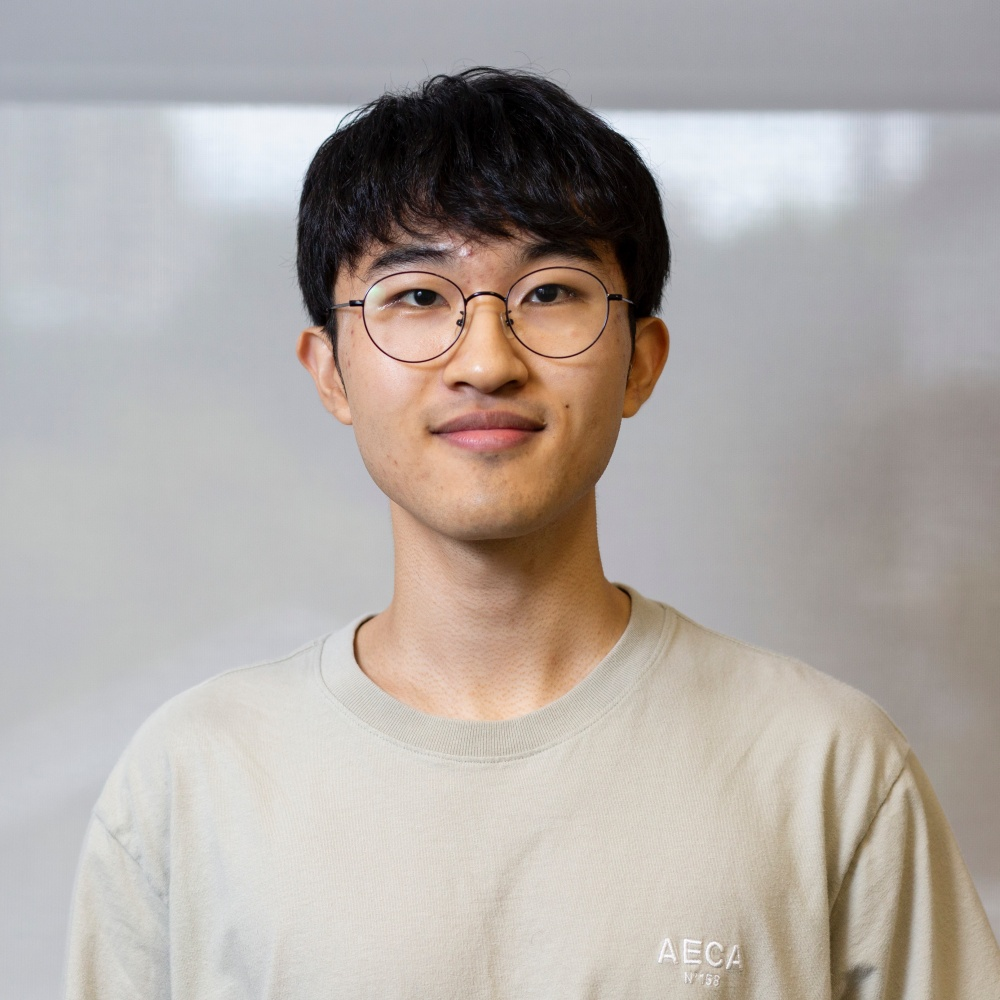
\includegraphics[width=0.3\textwidth]{photo.jpg}} &
		\centerline{\textbf{{\LARGE Hyoungjoo Kim}}}
		\vspace{20pt}
		\centerline{\href{mailto:hyoungjoo@cmu.edu}{hyoungjoo@cmu.edu}}
		\vspace{10pt}
		\centerline{\url{https://hyoungjook.github.io}}
		\vspace{10pt}
		\centerline{
			\LARGE
			\href{https://scholar.google.com/citations?user=sYhlQ1YAAAAJ&hl=en}{\faicon{graduation-cap}} \quad
			\href{https://www.linkedin.com/in/hyoungjoo-kim-546986194}{\faicon{linkedin}} \quad
			\href{https://github.com/hyoungjook}{\faicon{github}}
		} & \\
	\end{tabular}
\end{center}

\section{Research Interests}
I'm currently working on designing Databases for Processing-in-Memory Systems. \newline
In general, I'm interested in {\bf Software Systems \& Architecture} for {\bf Heterogeneous Devices}; e.g.
\begin{itemize}
	\item Database Systems for Processing-in-Memory
	\vspace{-5pt}
	\item Machine Learning Systems for GPU clusters
\end{itemize}

\section{Education}
\resumeSubHeadingListStart
	\resumeSubheading
		{\href{https://cmu.edu}{Carnegie Mellon University}}{Pittsburgh, Pennsylvania}{2023 - Present}
		{
			Ph.D. Student in Computer Science \newline
			Advisor: \href{https://www.cs.cmu.edu/~gibbons/}{Phillip B. Gibbons}
		}
	\resumeSubheading
		{\href{https://en.snu.ac.kr}{Seoul National University}}{Seoul, Korea}{2017 - 2023}
		{
			B.S. in Electrical and Computer Engineering \newline
			Advisor: \href{https://hpcs.snu.ac.kr/~jangwoo/}{Jangwoo Kim} \newline
			GPA: 4.28/4.3 \  (2nd/148) \newline
			{\small The period includes two years of mandatory military service in South Korea.}
		}
\resumeSubHeadingListEnd

\section{Honors and Awards}
\resumeSubHeadingListStart
\resumeSubheadingSimple{
	Overseas PhD Scholarship, Korea Foundation for Advanced Studies (KFAS)
}{2023 - 2028}
\resumeSubheadingSimple{
	The Presidential Science Scholarship, Korea Student Aid Foundation (KOSAF)
}{2017 - 2023}
	\resumeSubHeadingListStart
	\resumeSubheadingVerySimple{Tuition + 20M KRW ($\sim$20K USD), 4 years}
	\resumeSubHeadingListEnd
\resumeSubheadingSimple{
	Gold Medal, International Physics Olympiad
}{2016}
\resumeSubheadingSimple{
	Silver Prize, Samsung Humantech Paper Award (for high school students)
}{2016}
	\resumeSubHeadingListStart
	\resumeSubheadingVerySimple{5M KRW ($\sim$5K USD)}
	\resumeSubHeadingListEnd
\resumeSubHeadingListEnd

\section{Publications}
\resumeSubHeadingListStart
	\resumeSubheadingItem{
		Taebum Kim, \textbf{Hyoungjoo Kim}, Gyeong-In Yu, Byung-Gon Chun \newline
		\href{https://openreview.net/forum?id=HVKmLi1iR4}{\textbf{BPipe: Memory-Balanced Pipeline Parallelism for Training Large Language Models}} \newline
		\textit{International Conference on Machine Learning (ICML)}, 2023 \textit{(Oral Presentation)}
	}
	\resumeSubheadingItem{
		\textbf{Hyoungjoo Kim} \newline
		\href{https://snu-primo.hosted.exlibrisgroup.com/permalink/f/1qb4pk8/82SNU_INST21903413170002591}{\textbf{Modeling the GPU Instruction Scheduling Performance using Microbenchmarks}} \newline
		\textit{Bachelor's Thesis}, Advised by Jangwoo Kim, \textit{Seoul National University}, 2023 \  \href{https://github.com/hyoungjook/gpudiag/blob/master/documents/paper.pdf}{[Paper]}
	}

\resumeSubHeadingListEnd

\section{Research and Work Experiences}
\resumeSubHeadingListStart
	\resumeSubheading
		{\href{https://pdl.cmu.edu/index.shtml}{Parallel Data Lab}}{Pittsburgh, Pennsylvania}{2023 - Present}
		{
			Graduate Research Assistant
			\vspace{-5pt}
			\begin{itemize}
				\item {(In Progress) \textit{PIM-Friendly Database}: Designing fast and efficient DBMS for Processing-in-Memory Systems}
			\end{itemize}
		}
	\resumeSubheading
		{\href{https://friendli.ai}{FriendliAI}}{Seoul, Korea}{2022 - 2023}
		{
			Research Intern, Part-time
			\vspace{-5pt}
			\begin{itemize}
				\item {\textit{BPipe}: Accelerating the training of LLMs by rebalancing memory utilizations}
				\item {\textit{GPU Kernel Optimization}: Optimized CUDA kernels for training LLMs}
			\end{itemize}
		}
	\resumeSubheading
		{\href{https://hpcs.snu.ac.kr/}{High Performance Computer System Lab}}{Seoul, Korea}{2021}
		{
			Undergraduate Thesis Project Student
			\begin{itemize}
				\item {\textit{GPUDiag}: Modeling GPGPU microarchitecture using automated microbenchmarks}
				\item {\textit{Multi-GPU gem5}: Extend gem5-APU to support multiple GPUs}
			\end{itemize}
		}
	\resumeSubheading
		{\href{http://www.geolux.co.kr/en/}{Geolux}}{Seoul, Korea}{2017 - 2018}
		{
			Software Engineering Intern, Full-time, Only on summer/winter breaks
			\vspace{-5pt}
			\begin{itemize}
				\item {\textit{Pothole Detector}: Trained AI models to detect potholes from driveway videos}
			\end{itemize}
		}
\resumeSubHeadingListEnd

\section{Intra- and Extracurricular Projects}
\resumeSubHeadingListStart
	\resumeSubheadingSimple{
		\textit{Cache Simulator} for x64 binaries using pintool
	}{Fall 2023}
	\resumeSubheadingSimple{
		\textit{Linux Kernel Hacking} to impelement custom scheduler, lock, and file system
	}{Spring 2022}
	\resumeSubheadingSimple{
		\textit{Compiler Frontend} for custom grammar rules using lex and yacc
	}{Fall 2021}
	\resumeSubheadingSimple{
		\textit{CNN Accelerator} that can process conv, fc, and maxpool using Verilog and FPGA
	}{Fall 2021}
	\resumeSubheadingSimple{
		\textit{CPU Simulator} for pipelined CPU with branch predictor and cache using Verilog
	}{Spring 2019}
	\resumeSubheadingSimple{
		\textit{IoT System} on the car fender that alarms the driver of safety incidents
	}{2019}
	\resumeSubheadingSimple{
		\textit{IoT System} in the billiards ball that evaluates the cueing accuracy
	}{2018}
	\resumeSubheadingSimple{
		\textit{3D Territory Game} that adds 3D graphics to the given game logic
	}{Spring 2018}
	\resumeSubheadingSimple{
		\textit{Robotic Car} that follows the path and escape from the maze
	}{Fall 2017}
	\resumeSubheadingSimple{
		\textit{Robotic Arm} that mimics human arm movement
	}{2017}
	\resumeSubheadingSimple{
		\textit{Robotic Arm} using thermally-driven super-coiled-nylon artificial muscles
	}{2015 - 2016}
\resumeSubHeadingListEnd

\section{Teaching Experiences}
\resumeSubHeadingListStart
	\resumeSubheadingSimple{
		Teaching Assistant - Seoul National University, ``Operating Systems''
	}{Spring 2023}
\resumeSubHeadingListEnd

\section{Skills}
\resumeSubHeadingListStart
	\resumeSubheadingVerySimple{
		C, C++, Python, CUDA, Verilog, Java, Linux Kernel, PostgreSQL, PyTorch
	}
	\resumeSubheadingVerySimple{
		Computer Architecture, Databases, GPUs, Machine Learning Systems, Operating Systems, Simulation
	}
	\resumeSubheadingVerySimple{
		English: TOEFL (R30/L28/S23/W28), GRE (V164/Q170/A4.0)
	}
\resumeSubHeadingListEnd

\end{document}
